\chapter{Определение основных параметров реостатного тормоза}
\section{Расчет параметров тягового электродвигателя}

Рассчитываем ток двигателя в часовом и продолжительном режиме по формуле

\begin{equation}
  \label{eq:motor_current}
  I = \frac{P}{\eta \, U}, 
\end{equation}
где P - мощность на валу двигателя, Вт; $\eta$ - КПД; U - напряжение, в соответствующем режиме работы, В.

Для часового режима, по формуле \eqref{eq:motor_current}
\begin{equation*}
  I_{\text{ч}} = \frac{P_{\text{ч}}}{\eta_{\text{ч}} \, U} = \frac{810000}{0,945 \cdot 1000} = 857 \, \text{А}.
\end{equation*}

Для продолжительного режима
\begin{equation*}
  I_{\text{п}} = \frac{P_{\text{п}}}{\eta_{\text{п}} \, U} = \frac{760000}{0,946 \cdot 1000} = 803 \, \text{А}.
\end{equation*}

Рассчитываем значение кривой намагничивания в точке продолжительного режима по формуле
\begin{equation}
 \label{eq:cPhi_nom}
 c\,\Phi(I_{\text{п}}) = \frac{U - \left( R_a + R_f \right) \, I_{\text{п} }}{\omega_{\text{п}}},
\end{equation}
где $R_a$, $R_f$ - сопротивления, соответственно обмотки якоря и обмотки возбуждения, Ом; $\omega_{\text{п}}$ - угловая скорость вращения вала двигателя в продолжительном режиме, рад/с, рассчитываемая по формуле
\begin{equation}
 \label{eq:omega}
 \omega_{\text{п}} = \frac{\pi \, n_{\text{п}}}{30}, 
\end{equation}
где $n_{\text{п}}$ - частота вращения двигателя, об/мин.

Выполняем вычисления по формулам \eqref{eq:omega} и \eqref{eq:cPhi_nom}
\begin{equation*} 
 \omega_{\text{п}} = \frac{3,14 \cdot 1120}{30} = 117,3, \, \text{рад/с}
\end{equation*}

\begin{equation*}
 c\,\Phi(I_{\text{п}}) = \frac{1000 - \left( 0,007 + 0,03 \right) \, 803 }{117,3} = 8,2 \, \text{В} \cdot \text{с}
\end{equation*}

Для построения характеристики намагничивания тягового двигателя воспользуемся универсальной характеристикой намагничивания, которую можно выразить следующей аппроксимирующей зависимостью
\begin{equation}
 \label{eq:cPhi_norm}
 \frac{c\,\Phi\left(I_{\text{в}}\right)}{c\,\Phi\left(I_{\text{п}}\right)} = a_5 \, \left( \frac{I_{\text{в}}}{I_{\text{п}}} \right)^5 + a_4 \, \left( \frac{I_{\text{в}}}{I_{\text{п}}} \right)^4 + a_3 \, \left( \frac{I_{\text{в}}}{I_{\text{п}}} \right)^3 + a_2 \, \left( \frac{I_{\text{в}}}{I_{\text{п}}} \right)^3 + a_1 \, \frac{I_{\text{в}}}{I_{\text{п}}}, 
\end{equation}
где $a_5 = 0,09$, $a_4 = -0,66$, $a_3 = 1,97$, $a_2 = -3.00$ и $a_1 = 2,61$. Зависимость \eqref{eq:cPhi_norm} выражается графиком на рисунке~\ref{fig:cPhi_norm} и представляет собой нормированную (в безразмерных параметрах) кривую намагничивания.

\begin{figure}[H]
    \centering    
    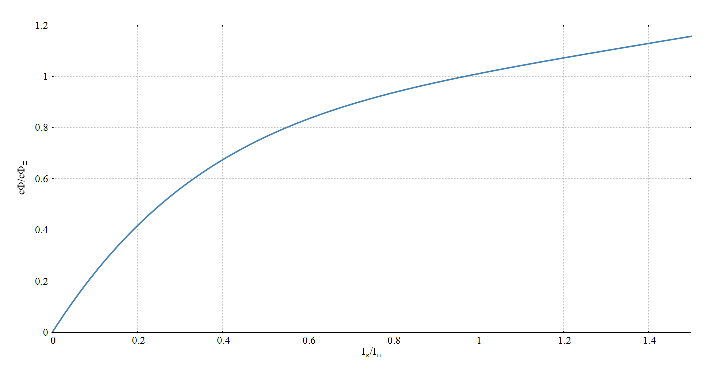
\includegraphics[width=0.7\textheight]{cPhi_norm.eps}
    \caption{Универсальная характеристика намагничивания ТЭД}
    \label{fig:cPhi_norm}
\end{figure}

Кривая намагничивания для конкретного, рассматриваемого нами двигателя, будет иметь вид
\begin{equation}
 \label{eq:cPhi}
 c\,\Phi\left(I_{\text{в}}\right) = b_5 \, I_{\text{в}}^5 + b_4 \, I_{\text{в}}^4 + b_3 \, I_{\text{в}}^3 + b_2 \, I_{\text{в}}^2 + b_1 \, I_{\text{в}},  
\end{equation}
где коэффициенты $b_1 - b_5$ расчитываются по формулам
\begin{equation}
 \label{eq:b_coeff}
 b_5 = \frac{c\,\Phi\left(I_{\text{п}}\right)}{I_{\text{п}}^5} \, a_5, \, b_4 = \frac{c\,\Phi\left(I_{\text{п}}\right)}{I_{\text{п}}^4} \, a_4, \, b_3 = \frac{c\,\Phi\left(I_{\text{п}}\right)}{I_{\text{п}}^3} \, a_3, \, b_2 = \frac{c\,\Phi\left(I_{\text{п}}\right)}{I_{\text{п}}^2} \, a_2, b_1 = \frac{c\,\Phi\left(I_{\text{п}}\right)}{I_{\text{п}}} \, a_1. 
\end{equation}

Рассчитываем коэффициенты кривой намагничивания по формулам \eqref{eq:b_coeff}, сводя результаты в таблицу~\ref{tab:b_coeff}
\begin{table}[H]
\centering
\caption{Коэффициенты аппроксимации кривой намагничивания}
\begin{tabular}{|c||c|c|c|c|c|}
 \hline
 k & 1 & 2 & 3 & 4 & 5 \\ \hline
 $a_k$ & 2,61 & -3,00 & 1,97 & -0,66 & 0,09 \\ \hline
 $b_k$ & 0,027 & $-3,81 \cdot 10^{-5}$ & $3,12 \cdot 10^{-8}$ & $-1,30 \cdot 10^{-11}$ & $2,21 \cdot 10^{-15}$ \\ \hline
\end{tabular}
\label{tab:b_coeff}
\end{table}

По формуле \eqref{eq:cPhi} рассчитываем значения кривой намагничивания для различных значений тока возбуждения, сводя результаты расчетов в таблицу~\ref{tab:tab_cPhi}

\begin{table}[H]
 \centering
 \caption{Точки кривой намагничивания тягового двигателя}
 \begin{tabular}{|c||c|c|c|c|c|c|c|c|c|c|}
  \hline
  $I_{\text{в}}$, А & 100 & 200 & 300 & 400 & 500 & 600 & 700 & 800 & 857 & 900 \\ \hline
  $c\Phi(I_{\text{в}})$, В$\cdot$с & 2,31 & 4,03 & 5,30 & 6,24 & 6,94 & 7,48 & 7,91 & 8,27 & 8,45 & 8,59  \\ \hline
 \end{tabular}
 \label{tab:tab_cPhi}
\end{table}
В таблице~\ref{tab:tab_cPhi} обязательно приводим значение характеристики намагничивания для часового тока ТЭД.

По данным таблицы~\ref{tab:tab_cPhi} строим график зависимости магнитного потока обмотки возбуждения от тока, протекающего через неё
\begin{figure}[H]
    \centering    
    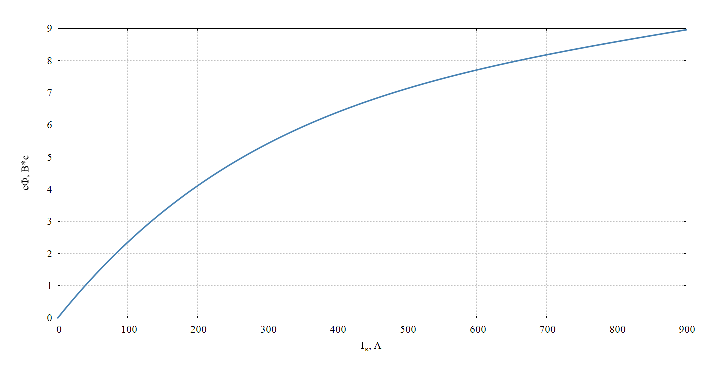
\includegraphics[width=0.7\textheight]{cPhi.eps}
    \caption{Характеристика намагничивания ТЭД}
    \label{fig:cPhi}
\end{figure}

\section{Построение предварительной тормозной характеристики}

Мощность реостатного тормоза принимаем равной продолжительной мощности электровоза, рассчитываемой по формуле
\begin{equation}
 \label{eq:power_reostat}
 P_{\text{т}} = n_a \, P_{\text{п}},
\end{equation}
где $n_a$ - число осей электровоза; $P_{\text{п}}$ - продолжительная мощность ТЭД. Для шестиосного пассажирского электровоза с заданными параметрами ТЭД
\begin{equation*}
 P_{\text{т}} = 6 \cdot 760 = 4560, \, \text{кВт}.
\end{equation*}

Принимаем в качестве ограничения тока якоря и тока возбуждения ТЭД,  при реостатном торможении, ток равный часовому току 857 А. Расчитываем момент, развиваемый тяговым двигателем при предельных значениях тока якоря и тока возбуждения
\begin{equation*}
 M_{\max} = c\Phi(I_{\text{ч}}) \, I_{\text{ч}} = 8,45 \cdot 857 = 7242, \, \text{Н} \cdot \text{м} 
\end{equation*}
Рассчитываем передаточное число осевого редуктора по формуле
\begin{equation}
 \label{eq:reductor}
 i_p = \frac{1,8 \, D_k \, \omega_{\max}}{v_k},
\end{equation}
где $D_k$ - диаметр бандажа по кругу катания, м; $\omega_{\max}$ - максимальная угловая скорость вращения тягового двигателя, рад/с; $v_k$ - конструкционная скорость электровоза, км/ч. Максимальная угловая скорость вращения ТЭД вычисляется по формуле \eqref{eq:omega}
\begin{equation*}
 \omega_{\max} = \frac{3,14 \cdot 2100}{30} = 220, \, \text{рад/с},
\end{equation*}
тогда
\begin{equation*}
 i_p = \frac{1,8 \cdot 1,25 \cdot 220}{160} = 3,09
\end{equation*}
Момент, приложенный к одной колесной паре электровоза
\begin{equation*}
 M_{\text{кп}} = i_p \, M_{\max} = 3,09 \cdot 7242 = 22378, \, \text{Н} \cdot \text{м},
\end{equation*}
Тогда, максимальное усилие, развиваемое реостатным тормозом
\begin{equation*}
 B_{\max} = \frac{M_{\text{кп}} \, n_a}{ 500 \, D_k} \,  = \frac{22378 \cdot 6}{500 \cdot 1,25} = 215, \, \text{кН} 
\end{equation*}
Скорость электровоза, при которой достигается максимальное тормозное усилие находим из условия постоянства мощности, рассеиваемой на тормозных резисторах
\begin{equation*}
 v_{B_{\max}} = \frac{3,6 \, P_{\text{т}}}{B_{\max}} = \frac{3,6 \cdot 4560}{215} = 76, \text{км/ч} 
\end{equation*}
Ветвь тормозной характеристики, при регулировании тока в обмотке возбуждения рассчитываем по формуле
\begin{equation}
 \label{eq:field_reg}
 B = \frac{3,6 \, P_{\text{т}}}{v}
\end{equation}
где $v$ - скорость электровоза, км/ч, в диапазоне от $v_{B_{\max}}$ до конструкционной скорости. Результаты расчета сводим в таблицу~\ref{tab:field_reg}

\begin{table}[H]
 \centering
 \caption{Ограничение по мощности тормозных резисторов}
 \begin{tabular}{|c||c|c|c|c|c|c|c|c|c|}
  \hline
  v, км/ч & 76 & 90 & 100 & 110 & 120 & 130 & 140 & 150 & 160 \\ \hline
  B, кН & 215 & 182 & 164 & 149 & 137 & 126 & 117 & 109 & 103 \\ \hline 
 \end{tabular}
 \label{tab:field_reg}
\end{table}

При предельном токе возбуждения и неизменном сопротивлении тормозных резисторов, тормозное усилие снижается линейно, пропорционально снижению скорости по закону
\begin{equation}
 \label{eq:linear_reg}
 B = B_{\max} \, \cfrac{v}{v_{B_{\max}}}
\end{equation}
Расчитываем линейную часть тормозной характеристики по формуле \eqref{eq:linear_reg} для диапазона скоростей от 0 до $v_{B_{\max}}$, сведя результаты в таблицу 

\begin{table}[H]
 \centering
 \caption{Линейная часть тормозной характеристики}
 \begin{tabular}{|c||c|c|c|c|c|c|c|c|}
  \hline
  v, км/ч & 0 & 10 & 20 & 30 & 40 & 50 & 60 & 76 \\ \hline
  B, кН & 0 & 28 & 56 & 84 & 112 & 141 & 169 & 215 \\ \hline 
 \end{tabular}
 \label{tab:linear_reg}
\end{table}












